\documentclass[review]{elsarticle}

\usepackage{lineno,hyperref}
\usepackage{pdflscape}
\modulolinenumbers[5]

\journal{Geochemica and Cosmochemica Acta}

%%%%%%%%%%%%%%%%%%%%%%%
%% Elsevier bibliography styles
%%%%%%%%%%%%%%%%%%%%%%%
%% To change the style, put a % in front of the second line of the current style and
%% remove the % from the second line of the style you would like to use.
%%%%%%%%%%%%%%%%%%%%%%%

%% Numbered
%\bibliographystyle{model1-num-names}

%% Numbered without titles
%\bibliographystyle{model1a-num-names}

%% Harvard
\bibliographystyle{model2-names.bst}\biboptions{authoryear}

%% Vancouver numbered
%\usepackage{numcompress}\bibliographystyle{model3-num-names}

%% Vancouver name/year
%\usepackage{numcompress}\bibliographystyle{model4-names}\biboptions{authoryear}

%% APA style
%\bibliographystyle{model5-names}\biboptions{authoryear}

%% AMA style
%\usepackage{numcompress}\bibliographystyle{model6-num-names}

%% `Elsevier LaTeX' style
%\bibliographystyle{elsarticle-num}
%%%%%%%%%%%%%%%%%%%%%%%

\begin{document}

\begin{frontmatter}

\title{Hydrous melting and partitioning in and above the mantle transition zone: insights from water-rich MgO-SiO$_2$-H$_2$O experiments}
%\tnotetext[mytitlenote]{Fully documented templates are available in the elsarticle package on \href{http://www.ctan.org/tex-archive/macros/latex/contrib/elsarticle}{CTAN}.}

%% Group authors per affiliation:
\author{R. Myhill, D. J. Frost}
\address{Bayerisches Geoinstitut, Universit\"{a}t Bayreuth, Universit\"{a}tsstrasse 30, 95447 Bayreuth, Germany}
\cortext[mycorrespondingauthor]{Corresponding author: R. Myhill}
\ead{myhill.bob@gmail.com}

\author{D. Novella}
\address{Laboratoire Magmas et Volcans, Universit\'{e} Blaise Pascal, 5 Rue Kessler, 63038 Clermond-Ferrand, France}

%% or include affiliations in footnotes:
%\author[mymainaddress,mysecondaryaddress]{Elsevier Inc}
%\ead[url]{www.elsevier.com}

%\author[mysecondaryaddress]{Global Customer Service\corref{mycorrespondingauthor}}

%\address[mymainaddress]{1600 John F Kennedy Boulevard, Philadelphia}
%\address[mysecondaryaddress]{360 Park Avenue South, New York}

\begin{abstract}

In this study, we conducted high pressure multianvil experiments at 13 GPa between 1200 and 1900 $^{\circ}$C to investigate the liquidus in the system MgO-SiO$_2$-H$_2$O. Water-rich starting compositions were obtained by using platinic acid (H$_2$Pt(OH)$_6$) as a novel water source. As MgO:SiO$_2$ ratios decrease, the liquidus curve develops an increasingly pronounced concave-down topology. At slab temperatures, the forsterite- and enstatite-water liquidii have similar water contents. Preliminary experiments on the SiO$_2$-H$_2$O binary reveal a pronounced melting point depression up to about 20 mol\% H$_2$O. This melting point depression exceeds estimates from published models, and requires either significant non-ideality between species in the melt, or distinct differences in the ease of protonation of bridging oxygens. We discuss the implications of this work on the migration of deep-seated slab fluids, and the partitioning of water between nominally anhydrous phases and melts.
\end{abstract}

\begin{keyword}
high pressure \sep mantle \sep hydrous melting \sep water \sep liquidus
\end{keyword}

\end{frontmatter}

\linenumbers

\section{Introduction}
Hydrous melts have a remarkable influence on Earth's surface and interior. Melting at subduction zones is primarily driven by the release of hydrous fluids from the warming slab at about 100 km depth, producing the world's arc volcanoes. The water cycle does not stop here, however; hydrous minerals within the crust should allow some water to be transported to 250 km \citep{PS2002}, and peridotite hydration should allow water to penetrate into the mantle transition zone or deeper, providing it remains low enough in temperature \citep{KOM2005}. This deep water cycle is probably the source for some kimberlitic eruptions, as implied by the discovery of water-saturated ringwoodite in a diamond from Juina, Brazil \citep{Pearsonetal2014}. The ringwoodite stability field requires that the kimberlite must have been sourced from at least ca. 500 km depth. In addition to kimberlites and arc volcanoes, hydrous melts are known to metasomatise and refertilise the lithospheric mantle, creating the so-called MARID (mica, amphibole, rutile, ilmenite, diopside) assemblage. It has also been argued that neutral or negatively buoyant water-rich melts are to blame for low velocity and high conductivity layers observed at the 410 km discontinuity, and that these small fraction melts could act to filter out incompatible elements during upwelling \citep{BK2003}. 

Processes involving deep-seated hydrous melts are controlled to a great extent by melt composition. Composition is a key variable in determining melt density, viscosity and solid-solid-melt dihedral angles, which together with the temperature and equivalent properties of the solid control the time- and lengthscales on which melt can separate from the melt. They also govern the extent to which this melt can become channelised, reducing interaction with its surroundings and increasing ascent rates. Melt compositions are also required to understand the stability of dense hydrous magnesium silicate (DHMS) phases and the water capacity of nominally anhydrous minerals (NAMS) at high pressure. Together, these control water transport and storage in the deep mantle, and as such are the primary inputs to models of the water budget of the Earth. Hydrous fluids at elevated pressures and temperatures cannot be treated as pure H$_2$O. As pressure increases, immiscibility between fluid and melt decreases, and the thermal stability of hydrous phases increases. As a result, fluids/melts released by the breakdown of hydrous phases have H$_2$O activities significantly lower than one. Understanding and predicting the \emph{P-T} conditions of DHMS phase breakdown and the water storage capacity at of NAMS therefore requires good activity-composition models for hydrous melts.


Constraining melt compositions remains a major challenge in high-pressure experimental petrology. The primary problem is that hydrous melts are unquenchable, which means that their water concentrations must be estimated indirectly. Compositions of partial hydrous melts have been estimated using a mixture of mass balance and defocused-beam electron probe measurements, which to provide Mg:Si ratios and a rough estimate of water content from deficits in totals. Such measurements are conducted on melt pockets \citep[e.g.][]{OMY2000, DDFK2005, LSOK2011} or melts isolated within diamond traps \citep{MSUP2007}. Unfortunately, these techniques are accompanied by significant uncertainties, especially in terms of water content. An alternative technique is to constrain the liquidus temperature at a given composition, thus circumventing the need to estimate water concentrations in the melt \emph{ex-situ} (when much of the water has been lost). The problem with this technique is that at ambient pressures, hydrous phases are limited in their maximum water content. For example, in the MgO-SiO$_2$ system, maximum water contents in a solid starting material are provided by a mixture of brucite and quartz. Thus, studies either extrapolate high temperature liquidus curves to high water contents or add water in liquid form. Extrapolation is prone to large errors, and accurately adding liquid water to the small volumes of high pressure capsules is essentially impossible. 

In this study, we use high purity platinic acid, hexahydroxyplatinate(IV) (H$_2$Pt(OH)$_6$), as a novel water source. Platinic acid is a pale yellow compound which is stable to about 130 $^{\circ}$C \citep{Nagano2002}. It breaks down at higher temperatures, releasing four molecules of H$_2$O and forming platinum (IV) oxide PtO$_2$. Its relatively high stability, high water content and the inert nature of the breakdown product (in a system where redox reactions are absent) make it an excellent water source for high pressure hydrous melting experiments.

\section{Experimental and analytical methods}
Starting compositions were created from a mixture of high-purity brucite, quartz and platinic acid (H$_2$Pt(OH)$_6$). Before weighing, quartz was dried at 1000 $^{\circ}$C for 12 hours, while brucite was heated to 250 $^{\circ}$C, also over 12 hours. Both powders were stored in a desiccating oven at 130 $^{\circ}$C. Platinic acid is hygroscopic, so was stored in a vacuum desiccator. Powders were weighed and ground dry in an agate mortar for 30 minutes, using a mask, goggles and gloves to avoid physical contact with the platinic acid. Starting compositions were stored in glass vials in a vacuum desiccator. Compositions are listed in Table \ref{table:compositions}.

\begin{table}[ht!]
\caption{Starting compositions}
\label{table:compositions}
\begin{tabular}{l|lll|lll}
 & \multicolumn{3}{c}{Oxide proportions (mol\%)} & \multicolumn{3}{|c}{Compound fractions (mol/mol)} \\
\hline
 & \multicolumn{1}{c}{MgO} & \multicolumn{1}{c}{SiO$_2$} & \multicolumn{1}{c}{H$_2$O} & \multicolumn{1}{|c}{Mg(OH)$_2$} & \multicolumn{1}{c}{SiO$_2$} & \multicolumn{1}{c}{H$_2$Pt(OH)$_6$} \\
\hline
br 5.0 & 50.000 & 0.000 & 50.000 & 1.000 & 0.000 & 0.000 \\
br 5.5 & 45.000 & 0.000 & 55.000 & 0.947 & 0.000 & 0.053 \\
br 6.0 & 40.000 & 0.000 & 60.000 & 0.889 & 0.000 & 0.111 \\
br 6.5 & 35.000 & 0.000 & 65.000 & 0.824 & 0.000 & 0.176 \\
br 7.0 & 30.000 & 0.000 & 70.000 & 0.750 & 0.000 & 0.250 \\
en 6.0 & 30.000 & 30.000 & 40.000 & 0.480 & 0.480 & 0.040 \\
en 7.0 & 26.667 & 26.667 & 46.667 & 0.457 & 0.457 & 0.086 \\
en 8.0 & 23.333 & 23.333 & 53.333 & 0.431 & 0.431 & 0.138 \\
en 9.0 & 20.000 & 20.000 & 60.000 & 0.400 & 0.400 & 0.200 \\
fo 11.5 & 36.000 & 18.000 & 46.000 & 0.637 & 0.319 & 0.044 \\
fo 13.0 & 32.000 & 16.000 & 52.000 & 0.604 & 0.302 & 0.094 \\
fo 14.5 & 28.000 & 14.000 & 58.000 & 0.566 & 0.283 & 0.152 \\
fo 16.0 & 24.000 & 12.000 & 64.000 & 0.522 & 0.261 & 0.217 \\
q 1.5 & 0.000 & 85.000 & 15.000	& 0.000	& 0.958	& 0.042 \\
q 2.0 & 0.000 & 80.000 & 20.000 & 0.000 & 0.941 & 0.059 \\
q 2.5 & 0.000 & 75.000 & 25.000 & 0.000 & 0.923 & 0.077 \\
q 3.0 & 0.000 & 70.000 & 30.000 & 0.000 & 0.903 & 0.097 \\
q 3.5 & 0.000 & 65.000 & 35.000 & 0.000 & 0.881 & 0.119 \\
q 4.0 & 0.000 & 60.000 & 40.000 & 0.000 & 0.857 & 0.143 \\
q 4.5 & 0.000 & 55.000 & 45.000 & 0.000 & 0.830 & 0.170 \\
q 5.0 & 0.000 & 50.000 & 50.000 & 0.000 & 0.800 & 0.200 \\
br+q 2.25 & 25.000 & 50.000 & 25.000 & 25.000 & 50.000 & 0.000 \\
br+q 2.70 & 30.000 & 40.000 & 30.000 & 30.000 & 40.000 & 0.000 \\
br+q 3.2 & 35.556 & 28.889 & 35.556 & 35.556 & 28.889 & 0.000 \\
br+q 3.4 & 37.778 & 24.444 & 37.778 & 37.778 & 24.444 & 0.000
\end{tabular}
\end{table}

Capsules were created from 2 mm-diameter Pt$_{90}$Rh$_{10}$ and Au rods, cut by wire saw into 1 mm thick disks. Into each disk were spark-eroded two rows of three holes, each 250 microns in diameter and 700 microns deep. The capsules were cleaned by cycling between an acetone ultrasonic bath (15 minutes) and 1000 $^{\circ}$C furnace (20 minutes) three times. Any remaining contamination was removed with a W$_{75}$Re$_{25}$ needle followed by a further trip to the ultrasonic bath. Capsule chambers were filled with powders of different compositions using a W$_{75}$Re$_{25}$ needle. Small pieces of tape were used to temporarily cover the other holes to avoid contamination. 

Multianvil experiments were performed in the 5000 tonne press at the Bayerisches Geoinstitut (BGI). Cr-doped MgO octahedral multianvil assemblies with 18 mm edge length were used (Figure \ref{fig:assembly}). Two capsules were loaded into each assembly, with the open ends of the chambers facing each other and separated by six 0.05 mm thick Pt$_{90}$Rh$_{10}$ or Au foils. The assemblies were compressed to 13 GPa over four hours between eight tungsten carbide cubes with trucations of edge-length 11 mm. Pressure calibrations and details of the press can be found in \cite{FPTLDR2004} and \cite{KF2005}. The assemblies were then resistively heated via the stepped LaCrO$_3$ heater. The temperature was recorded using a W$_{97}$Re$_{3}$--W$_{75}$Re$_{25}$ (Type D) thermocouple inserted axially into the assembly. To avoid water loss, higher temperature runs were heated for a shorter duration. The experiments were quenched by cutting power to the heater. The assemblies were then decompressed to room pressure over 1000 minutes. 

Capsules were recovered from the assembly, separated by wire saw and then ground by hand to reveal the tops of each capsule chamber. The wire saw was then used again to split the two sets of three chambers from each capsule. Each half-capsule was mounted in epoxy and mirror-polished. After revealing the edge of the capsule chambers, it was necessary to impregnate them with epoxy under vacuum before further polishing, in order to fill in the porous spaces created by the hydrous melt. Grinding under running water helped remove plucked grains from the polishing surface. Prepared and cleaned samples were then coated with a 10 nm thick carbon layer.

Analysis of run products was conducted via scanning electron microscope (SEM), using BSE imaging and EDS for phase identification (via the INCA software package). 

\section{Modelling water solubility in melts}

Oxygen in MgO-SiO$_2$-H$_2$O melts can exist either as molecular water, as a bridging oxygen between magnesium and/or silicon atoms, or as part of a terminal hydroxyl group. The general equation describing the reaction between melt species is
\begin{equation}
0.5 \textrm{H}_2\textrm{O} + 0.5 \textrm{O}_{br}^{2-} \rightleftharpoons \textrm{OH}_{tm}^-
\label{eqn:speciation}
\end{equation}

where the subscripts br and tm respectively refer to bridging and terminal oxygens. The equilibrium between these species can be described with an equilibrium constant $K$ \cite[e.g.][]{Stolper1982}
\begin{equation}
K = \frac{X_{\textrm{OH}_{tm}^-}}{\sqrt{X_{\textrm{H}_2\textrm{O}} X_{\textrm{O}_{br}^{2-}} } }
\label{eqn:equilibrium_constant}
\end{equation}

The equilibrium constant is related to the energy $\Delta G^{\circ}$ required to protonate a bridging oxygen
\begin{equation}
K = \exp\left(\frac{-\Delta G^{\circ}}{RT}\right)
\end{equation}

These equations can be used to describe in an average sense a range of melt-melt equilibria involving monomers (Mg(OH)$_2$ and Si(OH)$_4$), dimers (Mg$_2$O(OH)$_2$, MgSiO(OH)$_4$, Si$_2$O(OH)$_6$) and higher oligomers. A high proportion of monomers and dimers exist in relatively dilute solutions, but not in the concentrated solutions investigated in this study.

A number of models have been presented to investigate the behaviour of concentrated hydrous melts. \cite{SS1985} made the assumption that H$_2$O, O$_{br}^{2-}$ and OH$_{tm}^-$ mix ideally, with a parameter $r$ representing the number of oxygen atoms in each formula unit which are available for protonation. For example, an Mg$_2$SiO$_4$ melt with $r=4$ and $K=\infty$ represents a continuum between an anhydrous melt and one made of Mg(OH)$_2$ and Si(OH)$_4$ monomers. No distinction is made between isolated oligomers and partial depolymerisation of a silicate network; in other words, the energy required to form a terminal OH group is independent of local environment. Fixing $r$ places an implicit constraint on the maximum value of $K$ in water-rich compositions. For example, if $r=1$ in a hydrated MgO melt, then water contents exceeding 50 mol\% require that $K<\infty$. In practise, the equilibrium constant $K$ has been shown to be dependent on temperature and composition. \cite{SK1995} obtained a good fit to isochemical data with an expression of the form
\begin{equation}
\Delta G^{\circ} = a + b\,T
\end{equation}

\cite{THH2012} simplified the model of \cite{SS1985} by assuming that all hydrogen in the melt exists as OH$^-$, and that protonation is equally likely on any oxygen ($K=\infty$, $\Delta G^{\circ}=-\infty$, $r$ maximised). Deviations from this model must increase with increasing water content, and such a model cannot describe any melt more water-rich than the Mg(OH)$_2$-Si(OH)$_4$ binary. 

To describe melting in the SiO$_2$-H$_2$O system, \cite{HM2012} generalised the aforementioned models by allowing non-ideality between the two endmembers. The excess term $\Delta G^{\circ}$(P,T) for the formation of OH$^-$ groups was assumed to be independent of composition; all oxygens are equally available for protonation, and the local extent of protonation does not affect the energy required for each further protonation.

In these models, equilibrium melt compositions are calculated by calculating the activity of a component $x$ in the melt which has the composition of the anhydrous liquidus phase $X$ from the Gibbs energy of melting of $X$ at the temperature of interest:
\begin{equation}
RT \ln a_{x,L}^X = G_{X_l} - G_{X_{s}} = - \int_T^{T_{melt}} S_{X_{l}}-S_{X_s} \, dT
\end{equation}
where $T_{melt}$ is the temperature of melting of the liquidus phase under anhydrous conditions. 

In this study, we use a modified version of the molecular dynamics-derived anhydrous melt model of \cite{DKS2013} using melt endmembers MgO and SiO$_2$. For MgO melt, only the reference Helmholtz free energy needed to be adjusted. We note that the melting point of MgO at high pressure is rather uncertain. In the present model \citep{DKS2013}, MgO melts at $\sim$ 4180 K at 13 GPa, similar to that determined by previous ab-initio studies \citep{Alfe2005}. Experimental results vary by about 1000 K about this value \citep[3100 -- 5373 K at 13 GPa][]{ZB1994,ZF2008}. We note that if the present model is incorrect, it is probably the calculated entropy of melting which is at fault. A higher melting temperature would therefore imply a lower entropy of melting, such that the values in $G_{\textit{melt}}$ - $G_{\textit{solid}}$ at low temperatures will have smaller errors, than would otherwise be expected from such large melting point uncertainties. For the SiO$_2$ melt, the bulk modulus of the SiO$_2$ endmember was increased to satisfy the experimental constraint that coexisting melt and coesite have similar volumes at 13--14 GPa \citep{ZLGHF1993}. The volume at 1 bar is fit to experimental data. The entropy of melting at the coesite-stishovite-melt triple point ($\sim$40 J/K/mol) was kept the same. This value is identical to the value derived from the Clapeyron slope of the stishovite liquidus \cite{SL1995}. We note that this slope is much steeper than that recently proposed by \cite{Millotetal2015}. This difference is not the result of incompatibility between experimental results at different pressures \citep{SL1995, LAM1983, Millotetal2015}, but instead the result of using a 2-parameter Simon's equation to fit the rather abrupt change in dT/dP implied by the experiments at 20--40 GPa.

A subregular solution model was adopted to describe the free energy between the MgO and SiO$_2$ melts. The two interaction parameters W$_{MS}$ and W$_{SM}$ at 14 GPa were derived from the melt composition at the forsterite (fo)-HP clinoenstatite (hen) eutectic \citep{PWMW1998} and melting temperatures at the fo, hen and fo-hen cotectic compositions. The temperature dependence around 14 GPa was calculated by assuming an ideal excess entropy contribution, and then fitting to the known melting curves of forsterite and enstatite. The pressure dependencies were fit to the melting curves. It should be noted that although the excess volumes are similar to the results of \cite{DKS2013}, the excess entropies are some 50\% lower. However, they provide an excellent fit to the forsterite and orthoenstatite melting curves (see Supplementary Materials).

The calculations in the work were undertaken with the mineral physics toolkit Burnman \citep[available from \url{https://geodynamics.org/cig/software/burnman/}][]{CHRU2014}.

\clearpage
\section{Results}
\subsection{Ex-situ observations}
Experimental details and results are shown in Table \ref{table:experiments}. Superliquidus runs revealed networks of dendritic crystals of brucite, forsterite, enstatite and stishovite. Below the liquidus, solid phases tended to aggregate at the cold end of the capsules. Periclase formed equant crystals often associated with quench overgrowths which appear brighter in BSE images. Forsterite formed tabular crystals about 100 $\mu$m long. Enstatite crystals were much smaller, forming ca. 5 $\mu$m equant grains. Stishovite also formed equant to blocky grains, but crystals only separated from the melts in chambers with a high water content. In addition to the difference in texture and shape between quench crystals liquidus phases, subliquidus phases typically contained many small inclusions of Pt-Rh oxides. A typical set of run products is shown in Figure \ref{fig:sem}.

\begin{figure}[h!]
  \centering
      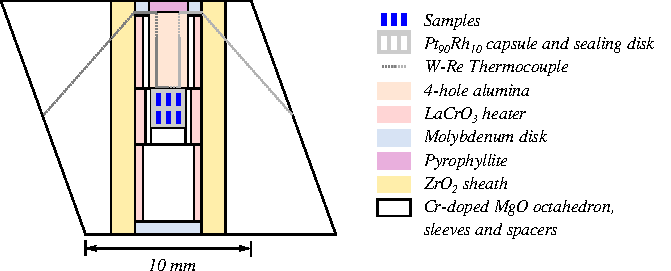
\includegraphics[width=0.8\textwidth]{figures/assembly}
  \caption{The 18/11 octahedral assembly design used in this study.}
  \label{fig:assembly}
\end{figure}

\begin{landscape}
\begin{table}[ht!]
\caption{Experimental run conditions and run products determined by SEM/EDS. Compositions are listed in order of increasing molar H$_2$O content. Unused compositions for each run are marked by an en-dash. Minor solids are listed in brackets. Mineral abbreviations are as follows: br - brucite, per - periclase, co - hydroxychondrodite, en - clinoenstatite, s - stishovite.}
\label{table:experiments}
\begin{tabular}{llllccccc}
Expt \# & P (GPa) & T ($^{\circ}$C) & t (min) & brucite+PtAc & forsterite+PtAcid & enstatite+PtAcid & quartz+PtAcid & br+q \\
Z1063 & 13 & 1200 & 40 & -/br/br/br/L & co/fo/fo/(fo) & en/en/en/en & -/-/-/-/-/-/-/- & -/-/-/- \\
Z1085 & 13 & 1300 & 40 & -/-/per/L/L & -/fo/(en)/L & -/-/-/- & -/-/-/-/-/-/-/- & -/-/-/- \\
Z1079 & 13 & 1300 & 35 & -/per/per/L/L & fo/fo/en/(en) & en/en/en/en & -/-/-/-/-/-/-/- & -/-/-/- \\
Z1058 & 13 & 1400 & 30 & -/per/(per)/L/L & fo/fo/L/L & en/en/en/(en) & -/-/-/-/-/-/-/- & -/-/-/- \\
Z1060 & 13 & 1500 & 20 & -/-/-/-/- & fo/L/L/L & en/en/L/L & -/-/-/-/-/-/-/- & -/-/-/- \\
Z1140 & 13 & 1600 & 10 & -/-/-/-/- & -/-/-/- & -/-/-/- & s/s/s/s/s/s/s/(s) & s+en/en/en/en \\
Z1084 & 13 & 1650 & 10 & -/-/-/-/- & -/-/-/- & L/L/-/- & -/-/-/-/-/-/-/- & -/-/-/- \\
Z1207 & 13 & 1700 & 8 & -/-/-/-/- & -/-/-/- & -/-/-/- & s/s/s/s/s/s/(s)/L & s+en/(en)/L/L \\
Z1209 & 13 & 1800 & 5 & -/-/-/-/- & -/-/-/- & -/-/-/- & s/s/s/s/(s?)/L/L/L & s/L/L/L \\
Z1091 & 13 & 1900 & 5 & (per)/-/-/-/- & -/-/-/- & -/-/-/- & -/-/-/L/-/L/L/L & L/L/-/-
\end{tabular}
\end{table}
\end{landscape}


\begin{figure}[ht!]
  \centering
      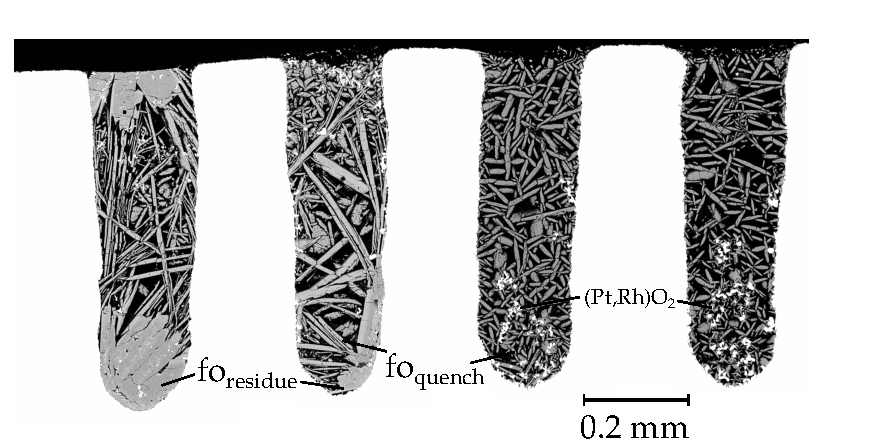
\includegraphics[width=0.8\textwidth]{figures/Z1058_1400C_13GPa_fo}
  \caption{BSE image of typical run products. Experimental chambers from Experiment Z1058, conducted at 1400 $^{\circ}$C and 13 GPa. Chambers have compositions along the forsterite-water binary, with water contents increasing from left to right.}
  \label{fig:sem}
\end{figure}


\subsection{Subsystems}
\subsubsection{MgO-H$_2$O}
The dehydration of brucite at high pressure was previously studied by \cite{FIYKFO2005}. They reported that the stability of brucite reaches a maximum at about 9--10 GPa and 1200 $^{\circ}$C, decomposing at 1100--1150 $^{\circ}$C at 13 GPa. We observed large brucite crystals at 1200 $^{\circ}$C and 13 GPa; the temperature difference is probably within experimental uncertainties. In the present study, the composition of the fluid coexisting with brucite and periclase is constrained to be 64--66 mol\% H$_2$O. The MgO content of the fluid increases gradually with increasing pressure, as a result of the extremely high melting temperature of periclase. 

Using the ideal OH$^-$ mixing model of \cite{SS1985} with no compositional dependence on the formation of OH groups, $G^{\circ}= -75000$ provides a good fit to the data if additional asymmetry is added via a binary subregular model (W$_{MgO-H_2O}$=55000 J/mol, W$_{H_2O-MgO}$=0 J/mol). This asymmetry is required to fit the activity of water at the periclase-brucite-liquid triple point to the solid thermodynamic models of \citep{HP2011} and the equation of state of water formulated by \cite{PS1995} ($0.52$). This model also has the effect of increasing the tendency for melt-fluid immiscibility at the water-rich end of the system. The second critical endpoint of the MgO-H$_2$O is probably around 13 GPa \citep{MSUP2007}, so large positive interaction enthalpies are justified in this region of the phase diagram. 

\begin{figure}[ht!]
  \centering
      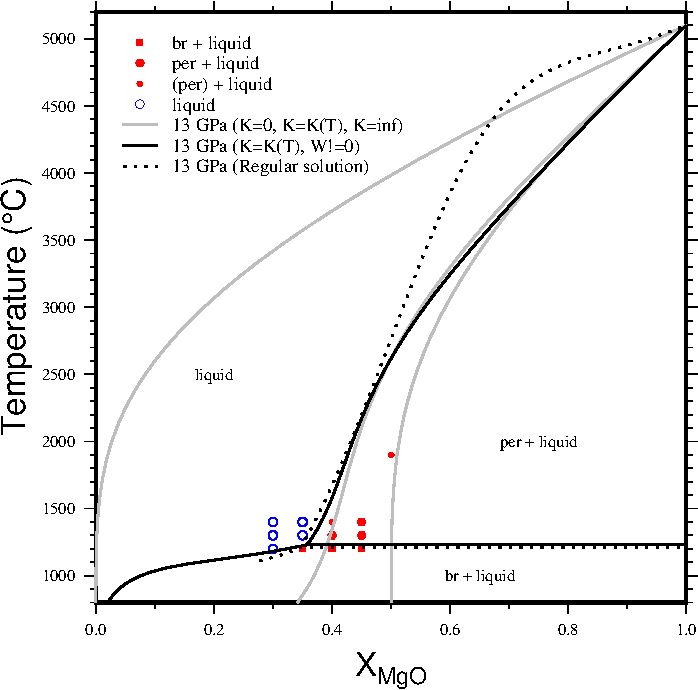
\includegraphics[width=0.8\textwidth]{figures/per-H2O}
  \caption{The periclase-water phase diagram at 13 GPa, based on current experimental results. The position of the dry periclase melting point is taken from \cite{ZF2008}, with an entropy of dry melting from \cite{CG1994}. Model fits in grey use the model of \cite{SS1985}, with r=1 and K=$\infty$ (bottom), K=K(T) (expression in main text) and K=0 (all H2O as molecular, top). The black line includes an interaction term to match the fluid in equilibrium with brucite during it's decomposition to periclase. The black dotted line represents a regular solution model with MgO, Mg(OH)$_2$ and H$_2$O as distinct species in the melt (parameters in the main text).}
  \label{fig:MH}
\end{figure}

\clearpage
\subsubsection{Mg$_2$SiO$_4$-H$_2$O}
The melting point depression of forsterite in the presence of water at 13 GPa is illustrated in Figure \ref{fig:foH}. The anhydrous melting of forsterite is incongruent. The temperature of the fo $\rightarrow$ per + L reaction is taken from \citep{PW1993}, with the temperature of the metastable fo $\rightarrow$ L reaction extrapolated from the same study. The liquidus is calculated by interpolation between the melting temperature of periclase \citep{ZF2008} and an estimate of the temperature and composition of melt in equilibrium with periclase and forsterite by interpolating between the invariant fo-per-foL point \citep{PW1993} and position of the per liquidus at 16 GPa \citep{LF2012}.

One chamber from an experiment run at 1300 $^{\circ}$C revealed a single very small crystal of enstatite. Another run at 1200 $^{\circ}$C revealed large crystals of hydroxychondrodite in the chamber with the lowest water contents. Small differences in Mg:Si ratio could explain the differences in solid phases between the separate chambers, so it is assumed that the enstatite+forsterite and chondrodite+forsterite cotectics cross the forsterite+H$_2$O binary at high water contents and 1200--1300 $^{\circ}$C. This supposition is supported by \cite{DDFK2005}, who observe a double-crossing of the liquid and wadsleyite-water tie-line at 15 GPa, first at ca. 1100 $^{\circ}$C, and again at 1400 $^{\circ}$C. Very similar Mg:Si ratios were observed by \citep{LSOK2011} at 15 and 18.5 GPa.

\begin{figure}[ht!]
  \centering
      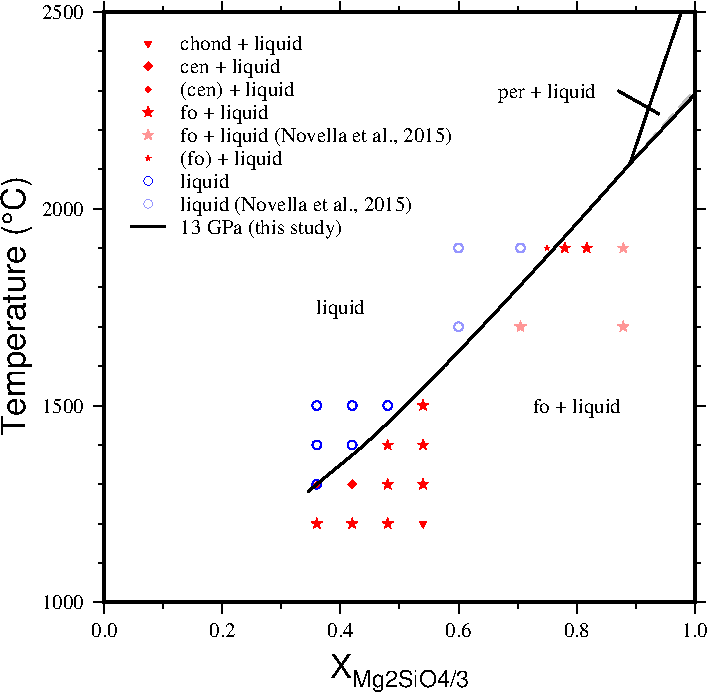
\includegraphics[width=0.8\textwidth]{figures/fo-H2O}
  \caption{The forsterite-water phase diagram at 13 GPa, based on current experimental results. The position of the dry melting point is taken from \citep{PW1993}. \citep{LF2012}.}
  \label{fig:foH}
\end{figure}
\clearpage
\subsubsection{MgSiO$_3$-H$_2$O}

The melting of clinoenstatite in the presence of water is shown in Figure \ref{fig:eoH}. The lack of stishovite as a liquidus phase is in agreement with \cite{YII2004}, who reported a clinoenstatite + stishovite + liquid field appearing at 13.5 GPa. 
\begin{figure}[ht!]
  \centering
      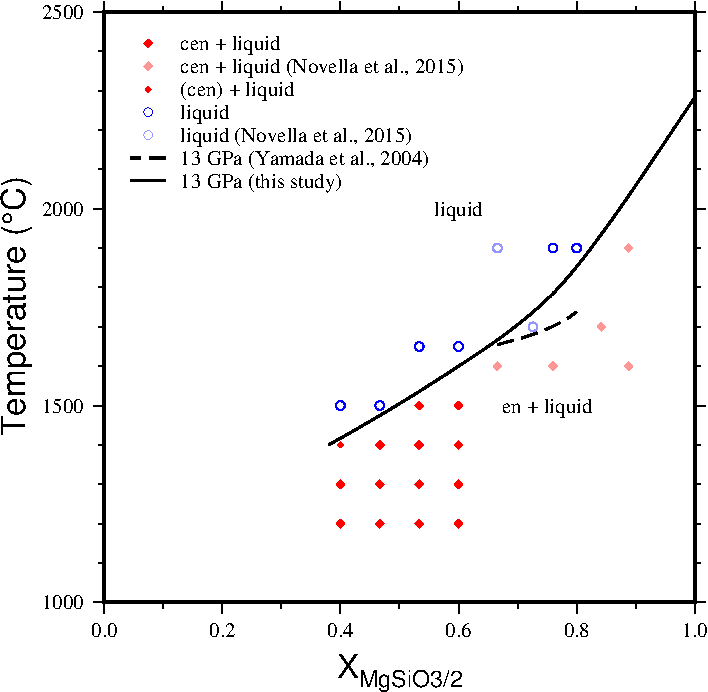
\includegraphics[width=0.8\textwidth]{figures/en-H2O}
  \caption{The clinoenstatite-water phase diagram at 13 GPa, based on current experimental results. The position of the dry melting point is taken from \cite{PG1990}.}
  \label{fig:eoH}
\end{figure}

\clearpage
\subsubsection{SiO$_2$-H$_2$O}
The 13 GPa SiO$_2$-H$_2$O binary phase diagram is shown in Figure \ref{fig:SH}. 

%NB: Most likely culprit the change in S with temperature?? Need a melt and solid model to test this.

% We use the formulation of \cite{HM2012} to model SiO$_2$-H$_2$O melts at 13 GPa. The volume of stishovite is taken from \cite{HP2011}. The melting curve of coesite at this pressure has $dT/dP \sim 0$ \citep{ZLGHF1993}, so the volume of anhydrous SiO$_2$ at this pressure is roughly equal to the volume of coesite via the Clausium-Clapeyron relation $dT/dP = \Delta V / \Delta S$. Using these volumes, the metastable entropy of melting of stishovite $\Delta S_{stv-L}$ is estimated as 8.5 J/K/mol. For completeness, we also calculate the melting point and entropy of melting of ice VII at 13 GPa from \emph{P-V-T} data collected along the melting curve \citep{FFH2004}.

\begin{figure}[ht!]
  \centering
      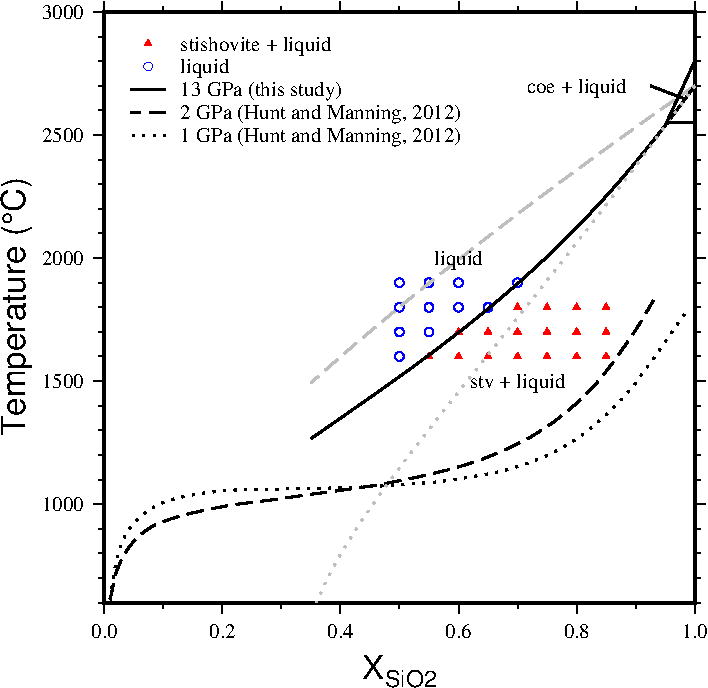
\includegraphics[width=0.8\textwidth]{figures/SiO2-H2O}
  \caption{The silica-water phase diagram at 13 GPa, based on current experimental results. The liquidus curve is compared with previous experimentally-derived models computed at 1 GPa and 2 GPa \citep{HM2012}. An entropy of 13.5 J/K/mol is chosen to fit the data. Model fits use the model of \cite{SS1985}, with r=2 and K=$\infty$ (dotted grey), K=K(T) (black, expression in main text) and K=0 (dashed grey, all H2O as molecular).}
  \label{fig:SH}
\end{figure}

%\citep{SU2001}
%\citep{KOM2005}
%\citep{AA1980}
%\citep{Wunder1998}
%\citep{AFRH2001}
%\citep{Nagano2002}
%\citep{MSUP2007}
%\citep{MFY2002}
%\citep{Sta2004}
%\citep{MFY2004}
%\citep{SUTG2001}
%\citep{NM2008}
%\citep{DM2010}
%\citep{ZK1998}

\clearpage
\subsection{The MgO-SiO$_2$-H$_2$O system}
The set of experimental run products can be used to create a preliminary liquidus diagram (Figure \ref{fig:liquidus}).

\cite{YII2004} suggested that there was a sharp break in the liquidus at the enstatite-stishovite cotectic (their Figure 6). However, this prediction breaks Schreinemakers Rules (specifically, that no one assemblage can occupy more than 180$^{\circ}$ around an invariant point).  


\begin{figure}[ht!]
  \centering
      \includegraphics[width=0.8\textwidth]{figures/experimental-ternary}
  \caption{A preliminary liquidus diagram at 13 GPa, based on current experimental results.}
  \label{fig:liquidus}
\end{figure}


\section{Discussion}
\subsection{Melting in the MgO-SiO$_2$-H$_2$O system}
\subsection{Water partitioning in the mantle transition zone}
% Olivine, wadsleyite and ringwoodite

Partitioning of hydrogen between mineral and melt phases can be described using a partition coefficient D:
\begin{equation}
  D^{a/b}_{H_2O} = c^a_{H_2O} / c^b_{H_2O}
\end{equation}
where $c^i_{H_2O}$ is the concentration of H$_2$O (in wt\%) in phase $i$ \citep{KB2006}. In quenchable phases, there are a number of ways that concentration can be measured, including FTIR, SIMS and ERDA. In the case of melts, which are unquenchable, $c^{melt}_{H_2O}$ in partitioning studies has most commonly been estimated by mass balance or by assuming that the deficit in microprobe totals is due to hydrogen. In two studies on Fe-free wadsleyite, \cite{DDFK2005} and \cite{LSOK2011} present estimates of water content in melts calculated from microprobe deficits. A similar study on ringwoodite was undertaken by \cite{OMY2000}. The T-X$_{H_2O}$ dependencies of the melts in equilibrium with wadsleyite or ringwoodite are strikingly different (Figure \ref{fig:partitioning}). For example, melt in equilibrium with wadsleyite at 15 GPa and 1400 $^{\circ}$C was estimated to contain 10.6-13.3 wt\% H$_2$O, while melt compositions in equilibrium with ringwoodite at 20 GPa and 1400 $^{\circ}$C suggest water contents of 57-66 wt\% H$_2$O. Modelled Mg$_2$SiO$_4$ melting temperatures increase by only 40 K between 15 and 20 GPa, and entropies of melting at these two pressures are not very different (92.4 vs. 97 J/K/mol), so unless the thermodynamics of mixing in the liquid change markedly between these pressures, estimates of $c^{melt}_{H_2O}$ for the ringwoodite or wadsleyite studies (or both) must be somewhat inaccurate. We note that two of the three melt compositions in equilibrium with ringwoodite fall above the temperatures indicating that hydrogen exists only as molecular H$_2$O \citep{SS1985}. In addition, the calculated liquidus temperatures in the wadsleyite studies at 15 GPa are lower than those reported at 5.5 GPa \citep{Inoue1994}. Both of these observations appear highly unlikely.

Here, we recalculate the wadsleyite/melt and ringwoodite/melt partitioning values with our melt model, assuming that the thermodynamic properties of the melt remain essentially constant between 13 and 20 GPa. Water concentrations in the solid are taken from the original studies. We restrict our analysis to data from 1100--1400 $^{\circ}$C, where the Mg:Si ratios of the melts are similar to that in forsterite. At 15 GPa, $D^{wad/melt}_{H_2O}$ increases from 0.30 to 0.51 between 900 and 1200 $^{\circ}$C, and then decreases back to 0.32 at 1400 $^{\circ}$C. The three ringwoodite H$_2$O concentrations (20-23 GPa) indicate a decrease in $D^{rw/melt}_{H_2O}$ from 0.68 to 0.57 between 1300 and ca. 1400 $^{\circ}$C.

\begin{figure}[ht!]
  \centering
      %\includegraphics[width=0.8\textwidth]{figures/partitioning}
  \caption{Water concentrations in wadsleyite, ringwoodite and melt, modelled at 15 and 20 GPa. Experimental data is taken from three published studies \citep{OMY2000,DDFK2005,LSOK2011}. Inset: Modelled partition coefficients between wadsleyite, ringwoodite and melt at 18 GPa.}
  \label{fig:partitioning}
\end{figure}

We now create a thermodynamic model for incorporation of H$_2$O into wadsleyite and ringwoodite. Hydrogen in wadsleyite and ringwoodite is incorporated as proton pairs substituting for Mg (Mg$^{2+}$ $\leftarrow$ 2H$^{+}$) \citep{Smyth1987, SHFJLM2003}. Ringwoodite potentially also exhibits a substitution involving Si (Si$^{4+}$ $\leftarrow$ Mg$^{2+}$ + 2H$^{+}$) \citep{KKMO2000}. Both of these reactions may be written in the form 
\begin{equation}
H_2O + O = (OH)_2
\end{equation}
which leads to the equilibrium relation 
\begin{eqnarray}
\Delta G = -R T \ln \left( \frac{a_{(OH)_2}}{a_{H_2O}a_{O}} \right), \\
= \Delta H - (T-T_0) \Delta S + (P-P_0) \Delta V
\end{eqnarray}
where $\Delta G$ is the Gibbs energy associated with the reaction. The second equation is a linearised form of the expression describing the change in free energy with pressure and temperature. The first equation can be simplified by making the approximation that $a_O$ is constant and that the weight percentage of H$_2$O in the solid $c_{H_2O}$ is proportional to the activity of (OH)$_2$. Both of these assumptions are probably reasonable at low values of $c_{H_2O}$. Rearranging now produces the expression:
\begin{equation}
c_{H_2O} \propto a_{H_2O} \exp{ \left( -\frac{\Delta H - (T-T_0) \Delta S + (P-P_0) \Delta V}{R T} \right) }
\end{equation}
Further simplifications can be made by taking $T_0 = 0$ K, by realising that $P_0$ can be neglected at high pressures, and by incorporating the factor $\Delta S/R$ into the exponential prefactor. Finally, it is recognised that the pressure and temperature dependence of the Gibbs free energy of water $G_{H_2O}$ is highly nonlinear. For this reason, we split the Gibbs free energy change of the anhydrous and hydrous solid from that of the liquid, yielding the equation \citep{KB2006}:
\begin{eqnarray}
c_{H_2O} = A a_{H_2O} f_{H_2O} \exp{ \left( -\frac{\Delta H + P \Delta V^{solid}}{R T} \right) }, \\
f_{H_2O} = \exp \left(\frac{\Delta G_{H_2O}}{RT} \right)
\end{eqnarray}

We calculate the fugacity of pure water $f_{H_2O}$ from the equation of state of \citep{PS1995}. We can now fit the values of A, $\Delta H$ and $\Delta V$ to the experimental data on wadsleyite and ringwoodite using our melt model. The pressure data of \cite{DDFK2005} at 1200 $^{\circ}$C and 14--17 GPa are consistent with a negligable pressure dependence on water content of wadsleyite, implying that $\Delta V \sim 10^{-5}$ m$^3$/mol, similar or slightly lower than estimates for olivine \citep[1.00 -- 1.06 $\cdot 10^{-5}$ m$^3$/mol][]{KKR1996, ZGK2004, MDAR2006}. A single data point at 18 GPa has much lower water contents, which would require $\Delta V \sim 1.25 \cdot 10^{-5}$ m$^3$/mol. This value is inconsistent with the large water contents at 16 and 17 GPa, and is probably unreasonable given the reported values for olivine. We therefore favour the lower estimate of $\Delta V$, and assume the same value for ringwoodite. The model values are shown in Table \ref{table:partitioning}.

\begin{table}[]
\centering
\caption{Thermodynamic models for water solubility in wadsleyite and ringwoodite}
\label{table:partitioning}
\begin{tabular}{lllll}
Phase & $P_{\textit{\tiny{ref}}}$ (Pa) & A [kg/(kgPa)] & $\Delta H_{P_{\textit{\tiny{ref}}}}$ [J/mol] & $\Delta V$ [m$^3$/mol] \\
\hline
Wadsleyite & 1.5e10 & 4.06e-12 & 1.66e5 & 1e-5 \\
Ringwoodite & 2.0e10 & 2.19e-12 & 2.04e5 & 1e-5 (fixed) \\
\end{tabular}
\end{table}


These models allow us to predict the partition coefficients of water between wadsleyite, ringwoodite and melt at the 520 km discontinuity ($\sim$18 GPa). $DD^{wad/ring}_{H_2O}$ increases from 0.6 at 1000 $^{\circ}$C to almost 1.0 at 2000 $^{\circ}$C. That these values are <1 indicate that water saturated peridotite in the lower mantle will partially melt during upwelling, which could explain observations of low velocity layers at ca. 520 km depth \citep[e.g.][]{JDH2010}. The small temperature dependence implies that repartitioning of water during secular cooling of the Earth is likely to be more minor (and in the opposite direction) to that proposed by \cite{DDFK2005}. 



\subsection{Deep water release from subduction zones}
% Densities
\cite{MF2010}
\cite{BK2003}
\cite{MSK2008}

% Viscosities
% Shear viscosity 
% Density

%So at least in my models there are three quantities that are important for the pattern of melt migration, the permeability, the compaction viscosity and the shear viscosity (if you have elasticity/plasticity, other things come in, too). Everywhere in the equations where you have the permeability, it's divided by the melt viscosity, and the permeability itself is normally assumed to scale with phi^3 (or less common phi^2), and at least I didn't see any parametrisations describing the effect of temperature on the permeability, so I would assume it's small. So for the permeability, you can just use the values you get for your different P-T-X conditions, and see if the overall term permeability/melt_viscosity increases or decreases.

%For the viscosities of the solid you have the influence of temperature on the viscosity (which I think is similar for shear and compaction viscosity) and you have the effect of porosity, eta ~ exp(alpa * phi) with phi~-27 for the shear viscosity (I think this is what Rich Katz uses in his models, but I would have to look it up to be sure), and xi ~ phi0/phi for the compaction viscosity, and you can do the same here, compare how they change for your different P-T-X conditions.


\section{Conclusions}



\clearpage
\section*{References}

\bibliography{references_MSH}

\end{document}
